\section{Preventivo}
La suddivisione oraria viene fatta tenendo conto del fatto che nel corso del progetto ogni  membro del gruppo deve ricoprire ogni ruolo almeno una volta.
Per facilitare la lettura delle successive tabelle sono state utilizzate le seguenti abbreviazioni per identificare i diversi ruoli:
\begin{itemize}
	\item \textbf{Re}: \textit{Responsabile};
	\item \textbf{Am}: \textit{Amministratore};
	\item \textbf{An}: \textit{Analista};
	\item \textbf{Pt}: \textit{Progettista};
	\item \textbf{Pm}: \textit{Programmatore};
	\item \textbf{Ve}: \textit{Verificatore};
\end{itemize}
Inoltre per determinare le ore nulle nelle successive tabelle verrà usato il simbolo -, che ne indica l'assenza.

\subsection{Fase di Analisi}
\subsubsection{Prospetto orario}
Nella fase di Analisi la distribuzione oraria è la seguente:
\begin{table}[H]
	\rowcolors{2}{lightest-grayest}{white}
	\centering
	\renewcommand{\arraystretch}{1.5}
	\begin{tabular}{|c|c|c|c|c|c|c|c|}
		\hline
		\rowcolor{lighter-grayer}
		Nome & Re & Am & An & Pt & Pm & Ve & Totale\\
		\hline
		
		% ----- Modificare da qui -----
		%  collegamento tabella a indice tabelle, dati;
		\hline
		\centering Badan Antonio & \centering - & \centering - & \centering 20 & \centering - & \centering - & \centering 16 & 36 \\
		\hline
		\centering Bertoldo Damiano & \centering - & \centering 20 & \centering - & \centering - & \centering - & \centering 16 & 36 \\
		\hline
		\centering Budai Matteo & \centering 10 & \centering - & \centering 20 & \centering - & \centering - & \centering 6 & 36 \\
		\hline
		\centering De Grandi Samuele & \centering 10 & \centering - & \centering 20 & \centering - & \centering - & \centering 6 & 36 \\
		 \hline
		\centering Piacere Ivan & \centering 10 & \centering - & \centering 20 & \centering - & \centering - & \centering 6 & 36 \\
		 \hline
		\centering Privitera Sara & \centering - & \centering 20 & \centering -& \centering - & \centering - & \centering 16 & 36 \\
		 \hline
		\centering Spigolon Daniele & \centering - & \centering 20 & \centering - & \centering - & \centering - & \centering 16& 36 \\
		 \hline
		\centering\textbf{Ore totali}  & \centering 30 & \centering 60 & \centering 80& \centering -  & \centering - & \centering 82 & 252 \\
		\hline
		
\end{tabular}
\caption*{\textbf{Tabella 2}: Distribuzione delle ore nella Fase di Analisi\\}
\end{table}	

I dati ottenuti possono essere riassunti nel seguente istogramma:
% fare istogramma (con dati poi), collegare all'indice delle figure;
\begin{figure}[H]
	\centering
	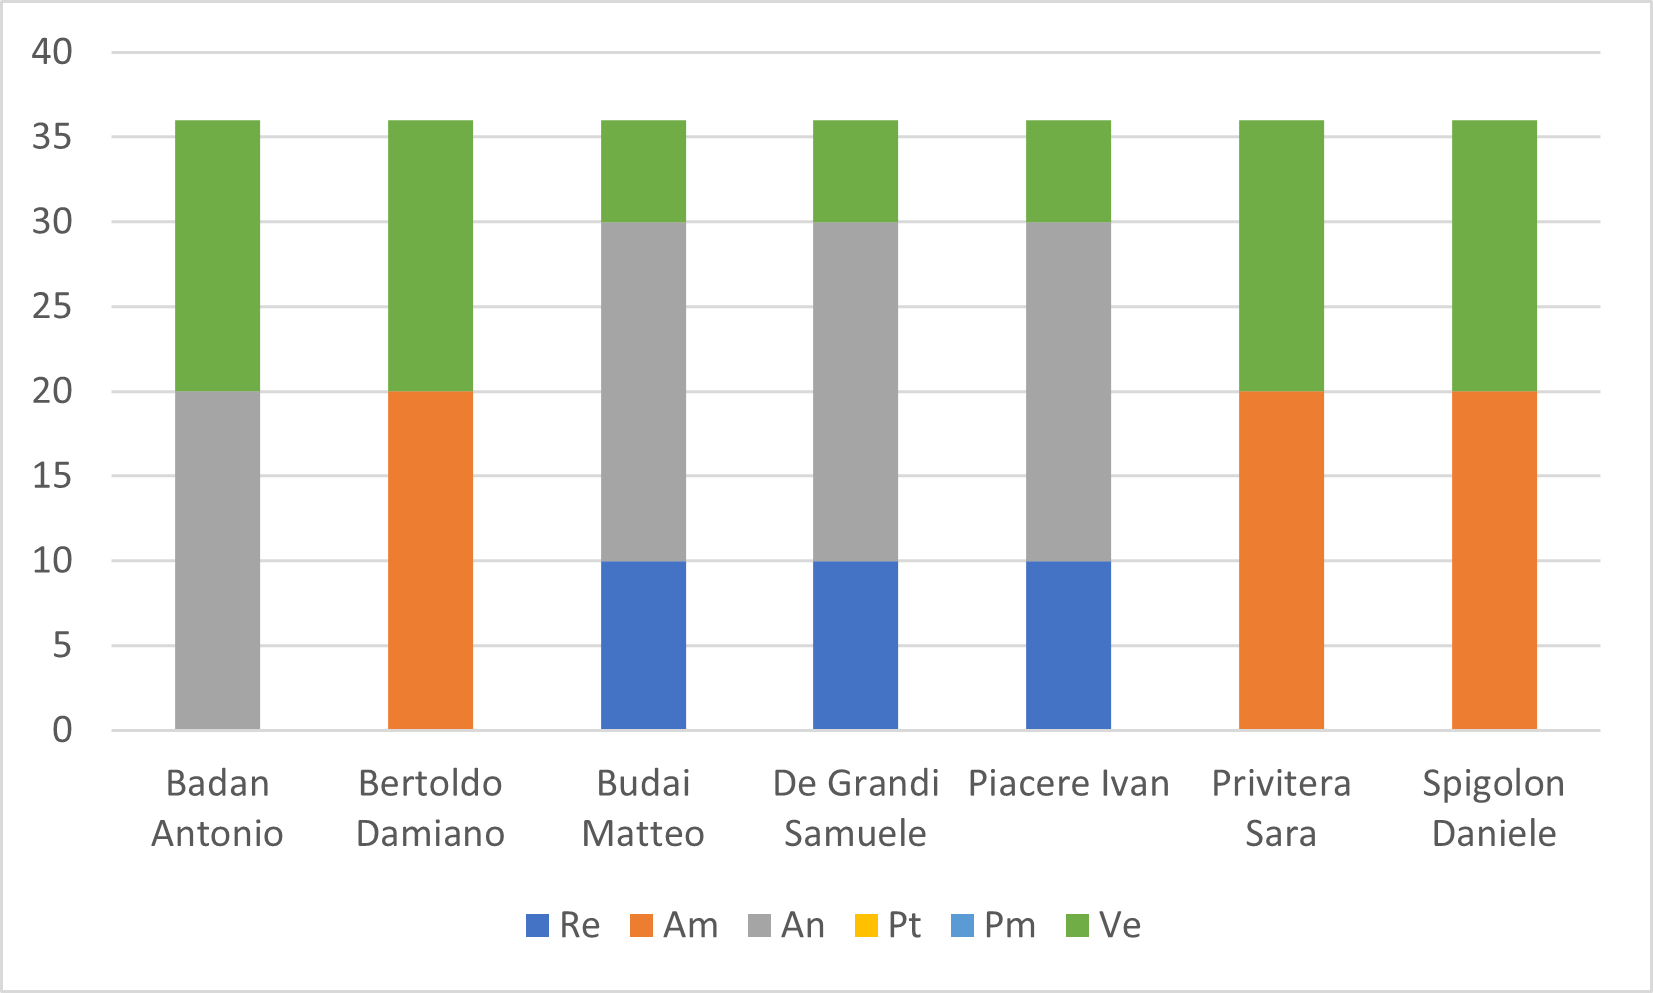
\includegraphics[width=0.7\linewidth]{res/images/Figura2.png}
	\caption*{\textbf{Figura2}: Istogramma della suddivisione delle ore durante la Fase di Analisi}
	\label{fig:Figura2}
\end{figure}

\subsubsection{Prospetto economico}
In questa fase il costo per ogni ruolo è il seguente:

\begin{table}[H]
	\rowcolors{2}{lightest-grayest}{white}
	\centering
	\renewcommand{\arraystretch}{1.5}
	\begin{tabular}{|c|c|c|}
		\hline
		\rowcolor{lighter-grayer}
		Ruolo & Ore & Costo\\
		\hline
		
		% ----- Modificare da qui -----
		%  collegamento tabella a indice tabelle;
		\centering Responsabile & \centering 30 & 900\euro\\ %30 per ora
		\hline
		\centering Amministatore & \centering 60 & 1200\euro\\ %20 per ora
		\hline
		\centering Analista & \centering 80 & 2000\euro\\ %25 per ora
		\hline
		\centering Progettista & \centering - & - \\ %22 per ora
		\hline
		\centering Programmatore & \centering - & - \\ %15 per ora
		\hline
		\centering Verificatore & \centering 82 & 1230\euro\\ %15 per ora
		\hline
		\centering\textbf{Totale} & \centering 252 & 5330\euro\\
		\hline
\end{tabular}
	\caption*{\textbf{Tabella 3}: Prospetto dei costi per ruolo nella Fase di Analisi\\}
\end{table}
I dati ottenuti possono essere riassunti nel seguente areogramma:
%collegare all'indice delle figure;
\begin{figure}[H]
	\centering
	\begin{tikzpicture}
		\pie{11.9/Responsabile, 23.8/Amministartore, 31.7/Analista, 32.5/Verificatore}
	\end{tikzpicture}
	\caption*{\textbf{Figura 3}:  Areogramma della ripartizione di ore per ruolo nella Fase di Analisi}
	\label{fig:Figura3}
\end{figure}	



\subsection{Fase di Progettazione architetturale}
\subsubsection{Prospetto orario}
Nella fase di Progettazione architetturale la distribuzione oraria è la seguente:

\begin{table}[H]
	\rowcolors{2}{lightest-grayest}{white}
	\centering
	\renewcommand{\arraystretch}{1.5}
	\begin{tabular}{|c|c|c|c|c|c|c|c|}
		\hline
		\rowcolor{lighter-grayer}
		Nome & Re & Am & An & Pt & Pm & Ve & Totale ore\\
		\hline
		Badan Antonio & 3 & 1 & 5 &  9 & - & 5 & 23 \\
		\hline
		Bertoldo Damiano & 3 & 1 & 5 & 9 & - & 5 & 23 \\
		\hline
		Budai Matteo & - & 1 & 6 & 10 & - & 6 & 23 \\
		\hline
		De Grandi Samuele & - & 1 & 6 & 10 & - & 6 & 23 \\
		\hline
		Piacere Ivan & - & 2 & 6 & 9 & - & 6 & 23 \\
		\hline
		Privitera Sara & 2 & 2 & 6 & 7 & - & 6 & 23 \\
		\hline
		Spigolon Daniele & 2 & 2 & 6 & 7 & - & 6 & 23 \\
		\hline
		Ore totali & 10 & 10 & 40 & 61 & - & 40 & 161 \\
		\hline
	\end{tabular}
	\caption*{\textbf{Tabella 4}: Distribuzione delle ore nel periodo di Progettazione architetturale\\}
\end{table}	
I dati ottenuti possono essere riassunti nel seguente istogramma:

\begin{figure}[H]
	\centering
	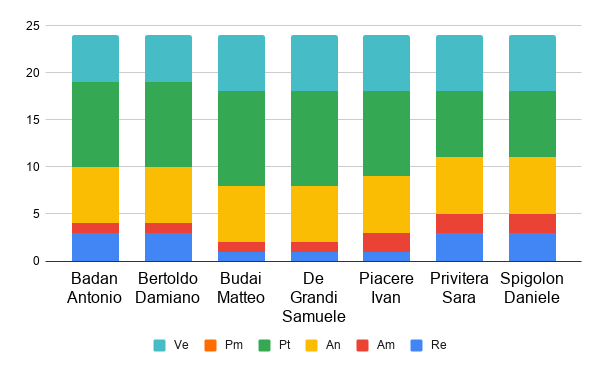
\includegraphics[width=0.7\linewidth]{res/images/IstogrammaFase2.png}
	\caption*{\textbf{Figura 4}: Istogramma della suddivisione delle ore durante il periodo di Progettazione architetturale}
	\label{fig:Figura10}
\end{figure}


\subsubsection{Prospetto economico}
In questa fase il costo per ogni ruolo è il seguente:

\begin{table}[H]
	\rowcolors{2}{lightest-grayest}{white}
	\centering
	\renewcommand{\arraystretch}{1.5}
	\begin{tabular}{|c|c|c|}
		\hline
		\rowcolor{lighter-grayer}
		Ruolo & Ore & Costo \\
		\hline
		Responsabile & 10 & 300\euro \\%30
		\hline
		Amministratore & 10 & 200\euro \\%20
		\hline
		Analista & 40 & 1000\euro \\%25
		\hline
		Progettista & 61 & 1331\euro \\%22
		\hline
		Programmatore & - & - \\%15
		\hline
		Verificatore & 40 & 600\euro \\%15
		\hline
		Totale & 161 &  3431\euro \\
		\hline
	\end{tabular}
	\caption*{\textbf{Tabella 5}: Prospetto dei costi per ruolo nel periodo di Progettazione architetturale\\}
\end{table}

I dati ottenuti possono essere riassunti nel seguente areogramma:


\begin{figure}[H]
	\centering
	\begin{tikzpicture}
		\pie{6.2/Responsabile, 6.2/Amministratore, 24.8/Analista, 37.9/Progettista, 24.8/Verificatore}
	\end{tikzpicture}
	\caption*{\textbf{Figura 5}: Areogramma della ripartizione di ore per ruolo in Progettazione architetturale}
	\label{fig:Figura10}
\end{figure}



\subsection{Fase di Progettazione di dettaglio e codifica}
\subsubsection{Prospetto orario}
Nella fase di Progettazione di dettaglio e codifica la distribuzione oraria è la seguente:

\begin{table}[H]
	\rowcolors{2}{lightest-grayest}{white}
	\centering
	\renewcommand{\arraystretch}{1.5}
	\begin{tabular}{|c|c|c|c|c|c|c|c|}
		\hline
		\rowcolor{lighter-grayer}
		Nome & Re & Am & An & Pt & Pm & Ve & Totale ore\\
		\hline
		Badan Antonio & 4 & 5 & 4 &  3 & 20 & 14 & 50 \\
		\hline
		Bertoldo Damiano & 4 & 5 & 4 & - & 20 & 17 & 50 \\
		\hline
		Budai Matteo & 5 & 6 & 4 & 5 & 20 & 10 & 50 \\
		\hline
		De Grandi Samuele & 4 & 6 & - & 5 & 20 & 15 & 50 \\
		\hline
		Piacere Ivan & 5 & 6 & - & 5 & 20 & 14 & 50 \\
		\hline
		Privitera Sara & 4 & 6 & 3 & - & 19 & 18 & 50 \\
		\hline
		Spigolon Daniele & 4 & 6 & 5 & 2 & 21 & 12 & 50 \\
		\hline
		Ore totali & 30 & 40 & 20 & 20 & 140 & 100 & 350 \\
		\hline
	\end{tabular}
	\caption*{\textbf{Tabella 6}: Distribuzione delle ore nel periodo di Progettazione di dettaglio e codifica\\}
\end{table}	
I dati ottenuti possono essere riassunti nel seguente istogramma:

\begin{figure}[H]
	\centering
	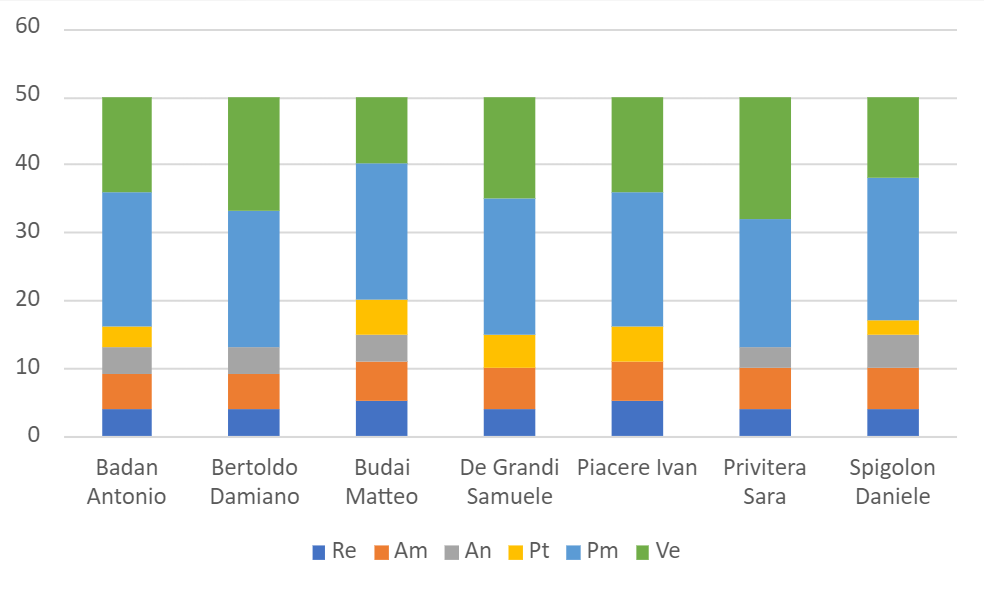
\includegraphics[width=0.7\linewidth]{res/images/IstogrammaFase3.png}
	\caption*{\textbf{Figura 6}: Istogramma della suddivisione delle ore durante il periodo di Progettazione di dettaglio e codifica}
	\label{fig:Figura10}
\end{figure}


\subsubsection{Prospetto economico}
In questa fase il costo per ogni ruolo è il seguente:

\begin{table}[H]
	\rowcolors{2}{lightest-grayest}{white}
	\centering
	\renewcommand{\arraystretch}{1.5}
	\begin{tabular}{|c|c|c|}
		\hline
		\rowcolor{lighter-grayer}
		Ruolo & Ore & Costo \\
		\hline
		Responsabile & 30 & 1050\euro \\%30
		\hline
		Amministratore & 40 & 800\euro \\%20
		\hline
		Analista & 20 & 125\euro \\%25
		\hline
		Progettista & 20 & 440\euro \\%22
		\hline
		Programmatore & 140 & 2250\euro \\%15
		\hline
		Verificatore & 100 & 1500\euro \\%15
		\hline
		Totale & 350 &  6165\euro \\
		\hline
	\end{tabular}
	\caption*{\textbf{Tabella 7}: Prospetto dei costi per ruolo nel periodo di Progettazione di dettaglio e codifica\\}
\end{table}

I dati ottenuti possono essere riassunti nel seguente areogramma:


\begin{figure}[H]
	\centering
	\begin{tikzpicture}
		\pie{8.6/Responsabile, 11.4/Amministratore, 5.7/Analista, 5.7/Progettista, 40/Programmatore, 28.6/Verificatore}
	\end{tikzpicture}
	\caption*{\textbf{Figura 8}: Areogramma della ripartizione di ore per ruolo in Progettazione di dettaglio e codifica}
	\label{fig:Figura10}
\end{figure}

\subsection{Fase di Validazione e collaudo}
\subsubsection{Prospetto orario}
Nella fase di Validazione e collaudo la distribuzione oraria è la seguente:

\begin{table}[H]
	\rowcolors{2}{lightest-grayest}{white}
	\centering
	\renewcommand{\arraystretch}{1.5}
	\begin{tabular}{|c|c|c|c|c|c|c|c|}
		\hline
		\rowcolor{lighter-grayer}
		Nome & Re & Am & An & Pt & Pm & Ve & Totale ore\\
		\hline
		Badan Antonio & 4 & 0 & 0 &  10 & 4 & 7 & 25 \\
		\hline
		Bertoldo Damiano & 6 & 0 & 0 & 0 & 10 & 9 & 25 \\
		\hline
		Budai Matteo & 0 & 9 & 0 & 0 & 5 & 11 & 25 \\
		\hline
		De Grandi Samuele & 0 & 7 & 0 & 5 & 4 & 9 & 25 \\
		\hline
		Piacere Ivan & 0 & 8 & 0 & 0 & 4 & 13 & 25 \\
		\hline
		Privitera Sara & 6 & 0 & 0 & 10 & 6 & 3 & 25 \\
		\hline
		Spigolon Daniele & 4 & 0 & 0 & 0 & 10 & 11 & 25 \\
		\hline
		Ore totali & 20 & 24 & 0 & 25 & 43 & 63 & 175 \\
		\hline
	\end{tabular}
	\caption*{\textbf{Tabella 9}: Distribuzione delle ore nel periodo di Validazione e collaudo\\}
\end{table}	
	I dati ottenuti possono essere riassunti nel seguente istogramma:

\begin{figure}[H]
	\centering
	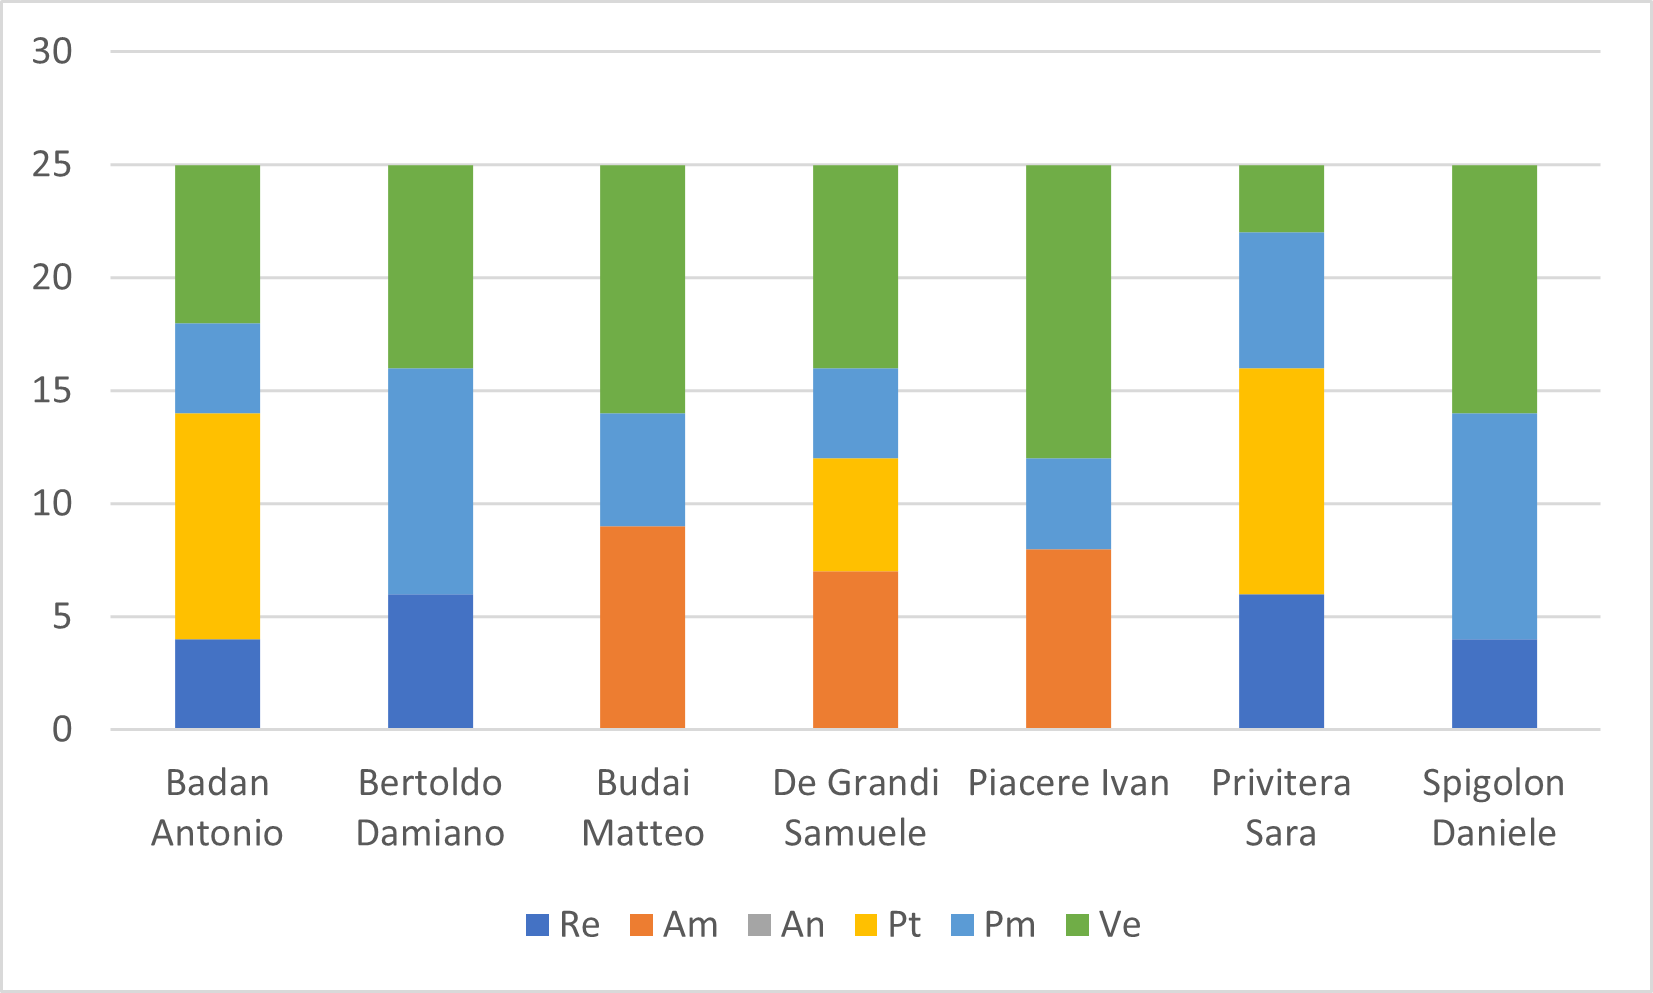
\includegraphics[width=0.7\linewidth]{res/images/Figura11.png}
	\caption*{\textbf{Figura 9}: Istogramma della suddivisione delle ore durante il periodo di Validazione e collaudo}
	\label{fig:Figura10}
\end{figure}
	
	
\subsubsection{Prospetto economico}
In questa fase il costo per ogni ruolo è il seguente:

\begin{table}[H]
	\rowcolors{2}{lightest-grayest}{white}
	\centering
	\renewcommand{\arraystretch}{1.5}
	\begin{tabular}{|c|c|c|}
		\hline
		\rowcolor{lighter-grayer}
		Ruolo & Ore & Costo \\
		\hline
		Responsabile & 20 & 620\euro \\
		\hline
		Amministratore & 24 & 504\euro \\
		\hline
		Analista & 0 & 0\euro \\
		\hline
		Progettista & 25 & 550\euro \\
		\hline
		Programmatore & 43 & 946\euro \\
		\hline
		Verificatore & 63 & 945\euro \\
		\hline
		Totale & 175 &  3565\euro \\
		\hline
	\end{tabular}
\caption*{\textbf{Tabella 10}: Prospetto dei costi per ruolo nel periodo di Validazione e collaudo\\}
\end{table}

I dati ottenuti possono essere riassunti nel seguente areogramma:


\begin{figure}[H]
	\centering
	\begin{tikzpicture}
		\pie{11.4/Responsabile, 13.7/Amministratore, 14.3/Progettista, 24.6/Programmatore,  36/Verificatore}
	\end{tikzpicture}
	\caption*{\textbf{Figura 10}: Areogramma della ripartizione di ore per ruolo in Validazione e collaudo}
	\label{fig:Figura10}
\end{figure}

\subsection{Riepilogo}
\subsubsection{Ore totali}
\paragraph{Prospetto orario totale}
Nella seguente tabella viene riportata la distribuzione oraria di tutte le fasi:

\begin{table}[H]
	\rowcolors{2}{lightest-grayest}{white}
	\centering
	\renewcommand{\arraystretch}{1.5}
	\begin{tabular}{|c|c|c|c|c|c|c|c|}
		\hline
		\rowcolor{lighter-grayer}
		Nome & Re & Am & An & Pt & Pm & Ve & Totale ore\\
		\hline
		Badan Antonio & 11 & 6 & 29 & 22 & 24 & 42 & 134 \\
		\hline
		Bertoldo Damiano & 13 & 26 & 9 & 9 & 30 & 47 & 134 \\
		\hline
		Budai Matteo & 15 & 16 & 30 & 15 & 25 & 33 & 134 \\
		\hline
		De Grandi Samuele & 14 & 14 & 26 & 20 & 24 & 36 & 134 \\
		\hline
		Piacere Ivan & 15 & 16 & 26 & 14 & 24 & 39 & 134 \\
		\hline
		Privitera Sara & 12 & 28 & 9 & 17 & 25 & 43 & 134 \\
		\hline
		Spigolon Daniele & 10 & 28 & 11 & 9 & 31 & 45 & 134 \\
		\hline
		Ore totali & 90 & 134 & 140 & 106 & 183 & 285 & 938 \\
		\hline
	\end{tabular}
	\caption*{\textbf{Tabella 11}: Prospetto orario che comprende tutte le fasi trattate in precedenza\\}
\end{table}	
I dati ottenuti possono essere riassunti nel seguente istogramma:

\begin{figure}[H]
	\centering
	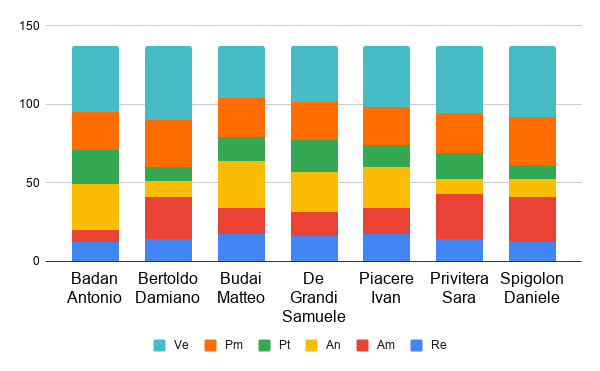
\includegraphics[width=0.7\linewidth]{res/images/IstogrammaTotale.png}
	\caption*{\textbf{Figura11}: Istogramma della suddivisione delle ore di tutte le fasi trattate in precedenza}
	\label{fig:Figura10}
\end{figure}

\paragraph{Prospetto economico totale}
Nella seguente tabella vengono mostrati i costi complessivi per ogni ruolo:

\begin{table}[H]
	\rowcolors{2}{lightest-grayest}{white}
	\centering
	\renewcommand{\arraystretch}{1.5}
	\begin{tabular}{|c|c|c|}
		\hline
		\rowcolor{lighter-grayer}
		Ruolo & Ore & Costo \\
		\hline
		Responsabile & 90 & 2870\euro \\
		\hline
		Amministratore & 134 & 2704\euro \\
		\hline
		Analista & 140 & 3125\euro \\
		\hline
		Progettista& 106 & 2321\euro \\
		\hline
		Programmatore & 183 & 3196\euro \\
		\hline
		Verificatore & 285 & 4275\euro \\
		\hline
		Totale & 938 &  18491\euro \\
		\hline
	\end{tabular}
	\caption*{\textbf{Tabella 12}: Prospetto dei costi totali per ciascun ruolo \\}
\end{table}

I dati ottenuti possono essere riassunti nel seguente areogramma:


\begin{figure}[H]
	\centering
	\begin{tikzpicture}
		\pie{9.6/Responsabile, 14.3/Amministratore, 14.9/Analista, 11.3/Progettista, 19.5/Programmatore,  30.4/Verificatore}
	\end{tikzpicture}
	\caption*{\textbf{Figura 12}: Areogramma dei costi totali delle ore di investimento e rendicontate}
    \label{fig:Figura10}
\end{figure}

\subsubsection{Ore totali rendicontate}
\paragraph{Prospetto orario totale rendicontato}
Nella seguente tabella viene riportata la distribuzione oraria di tutte le fasi a carico del committente, ad esclusione quindi, dell'Analisi e del Consolidamento dei requisiti:

\begin{table}[H]
	\rowcolors{2}{lightest-grayest}{white}
	\centering
	\renewcommand{\arraystretch}{1.5}
	\begin{tabular}{|c|c|c|c|c|c|c|c|}
		\hline
		\rowcolor{lighter-grayer}
		Nome & Re & Am & An & Pt & Pm & Ve & Totale ore\\
		\hline
		Badan Antonio & 11 & 6 & 9 & 22 & 24 & 26 & 98 \\
		\hline
		Bertoldo Damiano & 13 & 6 & 9 & 9 & 30 & 31 & 90 \\
		\hline
		Budai Matteo & 5 & 16 & 10 & 15 & 25 & 27 & 98 \\
		\hline
		De Grandi Samuele & 4 & 14 & 6 & 20 & 24 & 30 & 98 \\
		\hline
		Piacere Ivan & 5 & 16 & 6 & 14 & 24 & 33 & 98 \\
		\hline
		Privitera Sara & 12 & 8 & 9 & 17 & 25 & 27 & 98 \\
		\hline
		Spigolon Daniele & 10 & 8 & 11 & 9 & 31 & 29 & 98 \\
		\hline
		Ore totali & 60 & 74 & 60 & 106 & 183 & 203 & 686 \\
		\hline
	\end{tabular}
	\caption*{\textbf{Tabella 13}: Prospetto orario che comprende tutte le ore rendicontate\\}
\end{table}	
I dati ottenuti possono essere riassunti nel seguente istogramma:

\begin{figure}[H]
	\centering
	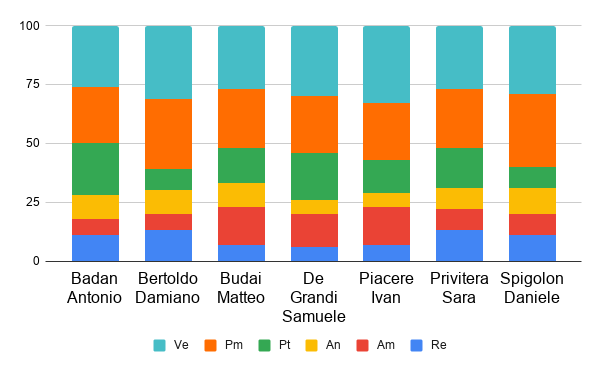
\includegraphics[width=0.7\linewidth]{res/images/IstogrammaTotaleRendicontato.png}
	\caption*{\textbf{Figura 13}: Istogramma della suddivisione delle ore rendicontate}
	\label{fig:Figura10}
\end{figure}

\paragraph{Prospetto economico totale rendicontato}
Nella seguente tabella vengono mostrati i costi complessivi rendicontati per ogni ruolo:

\begin{table}[H]
	\rowcolors{2}{lightest-grayest}{white}
	\centering
	\renewcommand{\arraystretch}{1.5}
	\begin{tabular}{|c|c|c|}
		\hline
		\rowcolor{lighter-grayer}
		Ruolo & Ore & Costo \\
		\hline
		Responsabile & 60 & 1970\euro \\
		\hline
		Amministratore & 74 & 1504\euro \\
		\hline
		Analista & 60 & 1125\euro \\
		\hline
		Progettista & 106 & 2321\euro \\
		\hline
		Programmatore & 183 & 3196\euro \\
		\hline
		Verificatore & 203 & 3045\euro \\
		\hline
		Totale & 686 &  13161\euro \\
		\hline
	\end{tabular}
	\caption*{\textbf{Tabella 14}: Prospetto dei costi totali rendicontati \\}
\end{table}

I dati ottenuti possono essere riassunti nel seguente areogramma:


\begin{figure}[H]
	\centering
	\begin{tikzpicture}
		\pie{8.7/Responsabile, 10.8/Amministratore, 8.7/Analista, 15.5/Progettista, 26.7/Programmatore, 29.6/Verificatore}
	\end{tikzpicture}
	\caption*{\textbf{Figura 14}: Areogramma delle ore rendicontate per ruolo}
    \label{fig:Figura10}
\end{figure}

\subsubsection{Conclusioni}
Il costo del progetto considerando le ore rendicontate è: 13161\euro.